\subsection{DQL -- Data Query Language}
\icode{SELECT} liest Daten aus einer oder mehreren Tabellen. Das Ergebnis ist immer wieder eine Tabelle (Mengeneigenschaft).

\subsubsection{Aufbau eines SELECT-Statements}
Die Schreibreihenfolge ist fest vorgegeben:
\begin{syntaxbox}[SQL]
SELECT   Spalten / Aggregatfunktionen
FROM     Tabellenname
WHERE    Bedingung          -- Zeilen filtern (VOR der Gruppierung)
GROUP BY Spalte             -- Gruppen bilden
HAVING   Bedingung          -- Gruppen filtern (NACH der Gruppierung)
ORDER BY Spalte ASC / DESC  -- Sortieren
LIMIT    Anzahl;            -- Anzahl begrenzen
\end{syntaxbox}

Die Schreibreihenfolge und die interne Ausführungsreihenfolge sind unterschiedlich:

\kzweispaltig{
\begin{stdtable}{l l}{Schritt & Befehl}
  1 & \icode{FROM} \\
  2 & \icode{WHERE} \\
  3 & \icode{GROUP BY} \\
  4 & \icode{HAVING} \\
  5 & \icode{SELECT} \\
  6 & \icode{ORDER BY} \\
  7 & \icode{LIMIT} \\
\end{stdtable}
}{
\begin{stdtable}{l X}{Begriff & Bedeutung}
  Horizontal & bestimmte \emph{Zeilen} filtern (\icode{WHERE}) \\
  Vertikal & bestimmte \emph{Spalten} auswählen (\icode{SELECT s1, s2}) \\
\end{stdtable}
}

\begin{syntaxbox}[SQL]
SELECT * FROM MA;                -- * = alle Spalten
SELECT VName, Gehalt FROM MA;    -- nur bestimmte Spalten (vertikal)
SELECT name AS Kundenname FROM kunde;  -- AS = Spalten-Alias
\end{syntaxbox}

\subsubsection{WHERE -- Zeilen filtern}
Mit \icode{WHERE} definiert man Einschränkungen (horizontales Filtern).

\begin{stdtable}{l X}{Operator & Bedeutung}
  \icode{>} / \icode{>=} & größer / größer gleich \\
  \icode{<} / \icode{<=} & kleiner / kleiner gleich \\
  \icode{=} & Gleichheit \\
  \icode{!=} oder \icode{<>} & ungleich \\
  \icode{AND} & beide Bedingungen müssen wahr sein \\
  \icode{OR} & mindestens eine Bedingung muss wahr sein \\
  \icode{NOT} & kehrt die Bedingung um \\
  \icode{XOR} & genau eine Bedingung darf wahr sein \\
\end{stdtable}

Klammern steuern die Reihenfolge der Auswertung:
\begin{syntaxbox}[SQL]
SELECT id_kunde, name FROM kunde
WHERE (ort = 'Muenster' OR YEAR(geb_datum) > 1960) AND id_kunde > 2;

-- BETWEEN: Bereich (inklusive Grenzen)
WHERE Gehalt BETWEEN 2000 AND 4000
-- entspricht: WHERE Gehalt >= 2000 AND Gehalt <= 4000

-- LIKE: Mustererkennung
WHERE VName LIKE 'M%'   -- beginnt mit M (% = beliebig viele Zeichen)
WHERE VName LIKE 'M_'   -- M + genau 1 Zeichen (_ = genau ein Zeichen)

-- IN: ersetzt eine Kette an OR-Bedingungen
WHERE AID IN (1, 2, 3)
-- entspricht: WHERE AID = 1 OR AID = 2 OR AID = 3
\end{syntaxbox}

\subsubsection{Funktionen}
Aggregatfunktionen fassen mehrere Zeilen zu einem einzelnen Wert zusammen. Sie arbeiten immer auf einer ganzen Spalte oder Gruppe. Daneben gibt es Zeichenketten- und Zeitfunktionen.

\begin{stdtable}{l X}{Funktion & Bedeutung}
  \icode{COUNT(*)} & Anzahl der Zeilen \\
  \icode{SUM(spalte)} & Summe aller Werte \\
  \icode{AVG(spalte)} & Durchschnitt aller Werte (\icode{NULL} wird ignoriert) \\
  \icode{MIN(spalte)} / \icode{MAX(spalte)} & kleinster / größter Wert \\
  \icode{LENGTH(s)} & Anzahl der Zeichen: \icode{LENGTH('frie')} $\rightarrow$ 4 \\
  \icode{LEFT(s, n)} / \icode{RIGHT(s, n)} & die ersten / letzten $n$ Zeichen einer Zeichenkette \\
  \icode{CURDATE()} / \icode{CURTIME()} & aktuelles Datum / aktuelle Uhrzeit \\
  \icode{CURRENT\_TIMESTAMP} & aktuelles Datum samt Uhrzeit \\
  \icode{YEAR(datum)} & Jahr eines Datums \\
\end{stdtable}

\begin{syntaxbox}[SQL]
SELECT
    COUNT(*)    AS AnzahlMitarbeiter,  -- AS vergibt einen Alias
    AVG(Gehalt) AS Durchschnittsgehalt,
    MIN(Gehalt) AS MinGehalt,
    MAX(Gehalt) AS MaxGehalt,
    SUM(Gehalt) AS Gesamtlohn
FROM MA;
\end{syntaxbox}

\subsubsection{GROUP BY und HAVING}
\icode{GROUP BY} fasst Zeilen mit dem gleichen Wert in einer Spalte zu einer Gruppe zusammen. Danach kann man pro Gruppe eine Aggregatfunktion anwenden. \icode{WHERE} filtert Zeilen \emph{vor} der Gruppierung, \icode{HAVING} filtert Gruppen \emph{nach} der Gruppierung.

\begin{syntaxbox}[SQL]
-- Ohne GROUP BY: ein Wert ueber alle Zeilen
SELECT AVG(Gehalt) FROM MA;

-- Mit GROUP BY: ein Wert pro Abteilung
SELECT AID, AVG(Gehalt) AS Durchschnittsgehalt
FROM MA
GROUP BY AID;

SELECT AID, COUNT(*) AS Anzahl
FROM MA
WHERE Gehalt > 2000       -- filtert Zeilen BEVOR Gruppen gebildet werden
GROUP BY AID
HAVING COUNT(*) > 2;      -- filtert Gruppen NACHDEM sie gebildet wurden
\end{syntaxbox}

\begin{merksatz}[Wichtige Regel]
Jede Spalte im \icode{SELECT}, die keine Aggregatfunktion ist, muss auch im \icode{GROUP BY} stehen -- sonst gibt es einen Fehler.
\end{merksatz}

\subsubsection{ORDER BY und LIMIT}
\begin{syntaxbox}[SQL]
SELECT VName, Gehalt FROM MA
ORDER BY Gehalt DESC;   -- DESC = absteigend, ASC = aufsteigend (Standard)

SELECT * FROM MA LIMIT 5;                  -- MySQL
SELECT * FROM MA FETCH FIRST 5 ROWS ONLY;  -- Standard-SQL
\end{syntaxbox}

\subsubsection{Joins}
Joins verknüpfen Daten aus mehreren Tabellen über eine Beziehung -- meist Primärschlüssel (Parent) = Fremdschlüssel (Child).

\begin{stdtable}{l X}{Join-Typ & Was wird ausgegeben?}
  \icode{INNER JOIN} & Nur Datensätze mit Treffer in \emph{beiden} Tabellen (Schnittmenge). \\
  \icode{LEFT JOIN} & Alle Datensätze der linken Tabelle -- auch ohne Treffer rechts. \\
  \icode{RIGHT JOIN} & Alle Datensätze der rechten Tabelle -- auch ohne Treffer links. \\
  \icode{CROSS JOIN} & Kartesisches Produkt: jede Zeile wird mit jeder kombiniert. \\
\end{stdtable}

\begin{figure}[H]
  \centering
  \begin{minipage}[b]{0.32\textwidth}
    \centering
    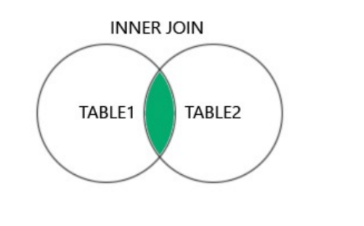
\includegraphics[width=\textwidth]{assets/images/InnerJoin}
  \end{minipage}\hfill
  \begin{minipage}[b]{0.32\textwidth}
    \centering
    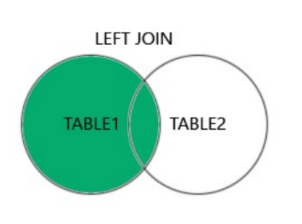
\includegraphics[width=\textwidth]{assets/images/LeftJoin}
  \end{minipage}\hfill
  \begin{minipage}[b]{0.32\textwidth}
    \centering
    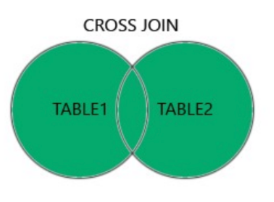
\includegraphics[width=\textwidth]{assets/images/CrossJoin}
  \end{minipage}
  \caption{Join-Typen als Schnittmengendiagramm: Inner Join, Left Join und Cross Join}
\end{figure}

\begin{syntaxbox}[SQL]
SELECT bestelldatum, name FROM kunde
INNER JOIN bestellung ON kunde.id_kunde = bestellung.id_kunde;
\end{syntaxbox}

\begin{infobox}[Merkhilfe: Schnittmengendiagramm]
\icode{INNER} = Überschneidung der beiden Kreise, \icode{LEFT}/\icode{RIGHT} = der ganze linke bzw. rechte Kreis. Vorsicht beim \icode{CROSS JOIN}: Das voll eingefärbte Diagramm steht hier für „alle Kombinationen“ -- ein Cross Join hat keine \icode{ON}-Bedingung und liefert bei $m$ und $n$ Zeilen $m \times n$ Ergebniszeilen. Die komplette Vereinigungsmenge beider Kreise wäre streng genommen ein \icode{FULL OUTER JOIN}.
\end{infobox}

\subsubsection{UNION}
Während ein Join Tabellen \emph{horizontal} verknüpft (Spalten nebeneinander), hängt \icode{UNION} die Ergebnisse zweier \icode{SELECT}-Abfragen \emph{vertikal} aneinander (Zeilen untereinander). Voraussetzung: Beide Abfragen müssen die gleiche Spaltenanzahl mit kompatiblen Datentypen liefern. \icode{UNION} entfernt dabei Duplikate, \icode{UNION ALL} behält sie.

\begin{syntaxbox}[SQL]
SELECT name, ort FROM kunde
UNION                              -- Duplikate werden entfernt
SELECT name, ort FROM lieferant;

SELECT name, ort FROM kunde
UNION ALL                          -- Duplikate bleiben erhalten
SELECT name, ort FROM lieferant;
\end{syntaxbox}

\begin{infobox}[FULL OUTER JOIN in MySQL]
MySQL kennt keinen \icode{FULL OUTER JOIN} -- man baut ihn mit \icode{UNION} nach: das Ergebnis eines \icode{LEFT JOIN} per \icode{UNION} mit dem Ergebnis des passenden \icode{RIGHT JOIN} vereinigen.
\end{infobox}

\subsubsection{Unterabfragen (Subselects)}
Wie in der Mathematik bei $f(g(x))$: Das innere Statement wird zuerst ausgeführt, sein Ergebnis nutzt die äußere Abfrage weiter. Das Ergebnis einer Unterabfrage ist immer eine Tabelle. Vorteil: Ein Teilproblem wird getrennt gelöst -- oft eine übersichtlichere Alternative zum Join.

\begin{syntaxbox}[SQL]
-- Unterabfrage im FROM (braucht immer einen Alias)
SELECT * FROM
    (SELECT VName FROM MA) AS temp;  -- AS temp ist Pflicht

-- Subselect im WHERE: zuerst MAX berechnen, dann damit vergleichen
SELECT VName, Gehalt FROM MA
WHERE Gehalt = (SELECT MAX(Gehalt) FROM MA);
\end{syntaxbox}

\subsubsection{Views (Sichten)}
Eine \emph{View} ist eine gespeicherte \icode{SELECT}-Abfrage, die wie eine virtuelle Tabelle genutzt wird. Im Unterschied zu einer Tabelle speichert eine View keine eigenen Daten, sondern nur die Abfrage -- die Daten liegen weiter in den Basistabellen.

\begin{procon}
  \pro{Komplexe Abfragen unter einem Namen speichern}
  \pro{Einheitliche Darstellung für alle Nutzer}
  \pro{Eingeschränkter, datensparsamer Zugriff}
  \con{Keine eigenen Daten -- Performance hängt an den Basistabellen}
\end{procon}
